\section{Hypothesis Tests}

\subsection{Fisher's Null Hypothesis Test}

\begin{frame}{Fisher's Null Hypothesis Test}

\structb{Overview.}
\begin{enumerate}
	\justifying
	\item Set up a \highlightg{null hypothesis} $H_0$ that compares a population para-meter $\theta$ to a given null value $\theta_0$.
	\begin{itemize}
		\item $H_0: \theta = \theta_0$,
		\item $H_0: \theta \leq \theta_0$,
		\item $H_0: \theta \geq \theta_0$.
	\end{itemize}
	\item Try to reject the null hypothesis by finding an upper bound (\highlightg{significance} or \highlightg{P-value}) of probability of obtaining the data or more extreme data (based on the null hypothesis), given that the null hypothesis is true.
	\begin{align*}
	P[D|H_0]\leq P-\U{valur}.
	\end{align*}
	\item We either 
	\begin{itemize}
		\item fail to reject $H_0$ or
		\item reject $H_0$ at the [p-value] level of significance.
	\end{itemize}
\end{enumerate}

\end{frame}

\begin{frame}{One-tailed Test}

\justifying
\structb{Null hypothesis.}
\begin{align*}
H_0: \theta \leq \theta_0 \qquad \U{or} \qquad H_0: \theta \geq \theta_0.
\end{align*}
\structb{Test for mean.} Suppose the sample mean $\overline{X}$ follows a normal distribution with mean $\mu$.
\begin{figure}[htbp]
	\centering
	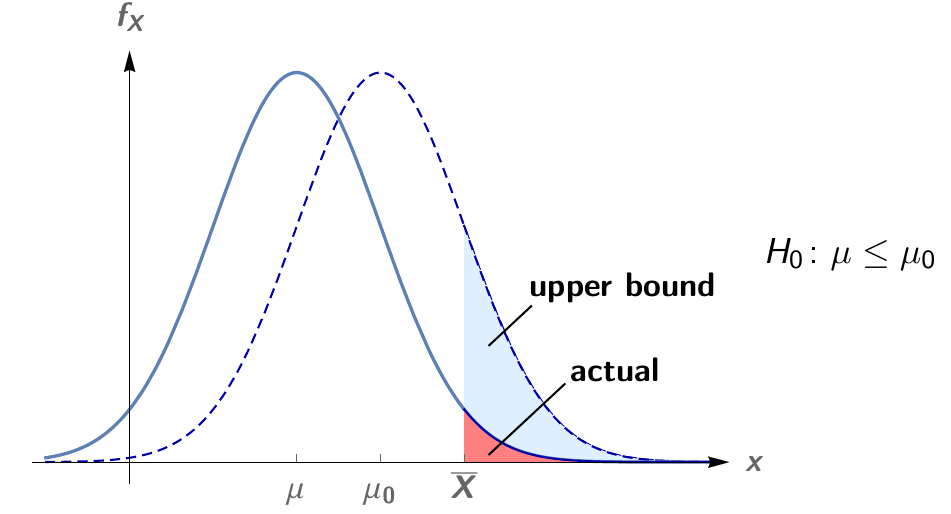
\includegraphics[width=8cm]{./images/rc5fig1.png}
\end{figure}

\end{frame}

\begin{frame}{Two-tailed Test}

\justifying
\structb{Null hypothesis.}
\begin{align*}
H_0: \theta = \theta_0.
\end{align*}
\structb{Test for mean.} Suppose the sample mean $\overline{X}$ follows a normal distribution with mean $\mu$.
\begin{figure}[htbp]
	\centering
	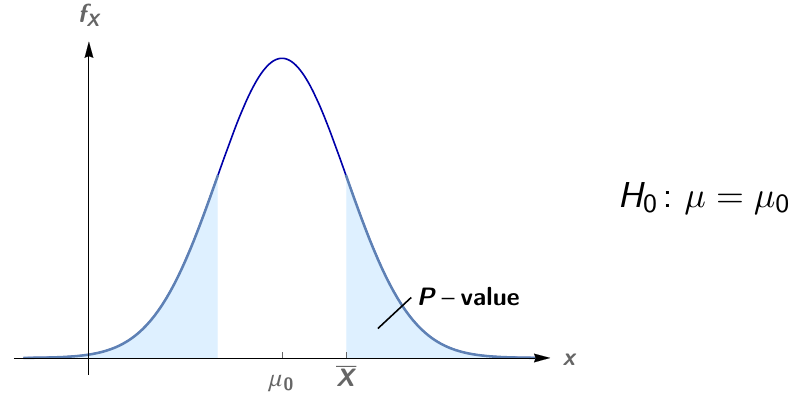
\includegraphics[width=8cm]{./images/rc5fig2.png}
\end{figure}

\end{frame}

\begin{frame}{Fisher's Null Hypothesis Test}

\structb{Example.}

\end{frame}


\subsection{Neyman-Pearson Decision Theory}

\begin{frame}{Neyman-Pearson Decision Theory}

\structb{Overview.}
\begin{enumerate}
	\justifying
	\item Set up a \highlightg{null hypothesis} $H_0$ and an \highlightg{alternative hypothesis} $H_1$.
	\item Determine a desirable $\alpha$ and $\beta$, where
	\begin{itemize}
		\item $\alpha := P[\U{accept\ } H_1|H_0 \U{\ true}]$, and
		\item $\beta := P[\U{accept\ } H_0|H_1 \U{\ true}]$.
	\end{itemize}
	\item Use $\alpha$ and $\beta$ to determine the appropriate sample size $n$. \highlightr{$\Delta$}
	\item Use $\alpha$ and $n$ to determine the critical region. \highlightr{$\Delta$}
	\item Obtain sample statistics, and reject $H_0$ at significance level $\alpha$ and accept $H_1$ if the test statistic falls into critical region. Otherwise, accept $H_0$.
\end{enumerate}

\end{frame}

\begin{frame}{Choosing the Sample Size}

\justifying
\structb{Special case.} Suppose the sample mean $\overline{X}$ follows a normal distri-bution with unknown mean $\mu$ and known variance $\sigma^2$, and we have hypothesis
\begin{align*}
H_0: \mu = \mu_0, \qquad H_1: |\mu - \mu_0| \geq \delta_0.
\end{align*}\\
\only<1>{
	\structb{Relation between $\alpha$, $\beta$ $\delta$, $\sigma$ and $n$.} With true mean $\mu = \mu_0 + \delta$, the test statistic $Z = \dfrac{\overline{X} - \mu_0}{\sigma/\sqrt{n}}\sim\U{N}(\delta\sqrt{n}/\sigma, 1)$.
	\begin{align*}
	P[\U{fail\ to\ reject\ } H_0|\mu = \mu_0 + \delta] & = \frac{1}{\sqrt{2\pi}}\int_{-z_{\alpha/2}}^{z_{\alpha/2}} e^{-(t-\delta\sqrt{n}/\sigma)^2/2} \U{d}t \\
	& = \frac{1}{\sqrt{2\pi}}\int_{-z_{\alpha/2}-\delta\sqrt{n}/\sigma}^{z_{\alpha/2}-\delta\sqrt{n}/\sigma} e^{-t^2/2}\U{d}t \\
	& \approx \frac{1}{\sqrt{2\pi}} \int_{-\infty}^{z_{\alpha/2}-\delta\sqrt{n}/\sigma} e^{-t^2/2}\U{d}t \overset{!}{=} \beta,
	\end{align*}
	giving $-z_{\beta} = z_{\alpha/2}-\delta\sqrt{n}/\sigma$.
}
\uncover<2>{
	\structb{Choosing the sample size $n$.}
	\begin{align*}
	n\approx \frac{(z_{\alpha/2} + z_{\beta})^2\sigma^2}{\delta^2},
	\end{align*}
	where $z_{\alpha/2}$ and $z_{\beta}$ satisfies that
	\begin{align*}
	\Phi(z_{\alpha/2}) = 1 - \alpha/2, \qquad \Phi(z_{\beta}) = 1 - \beta,
	\end{align*}
	given cumulative distribution function $\Phi$ of standard normal distribution.
}

\end{frame}


\begin{frame}{Choosing the Sample Size}

\structb{Special case.}
\begin{figure}[htbp]
	\centering
	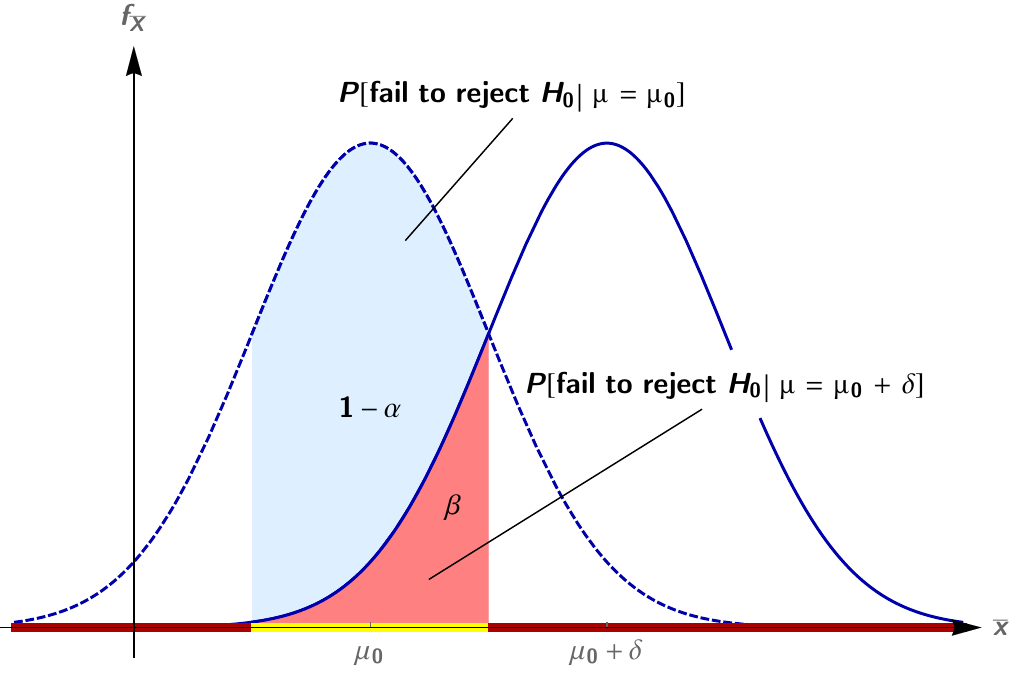
\includegraphics[width=8cm]{./images/rc5fig5.png}
\end{figure}

\end{frame}


\begin{frame}{Choosing the Sample Size}

\structb{More general case: OC curve.}
\begin{enumerate}
	\item Calculate
	\begin{align*}
	d := \frac{|\mu - \mu_0|}{\sigma}.
	\end{align*}
	\item Look up in OC curve for sample size $n$.
\end{enumerate}

\end{frame}


\begin{frame}{Choosing the Sample Size}

\structb{More general case: OC curve.}
\begin{figure}[htbp]
	\centering
	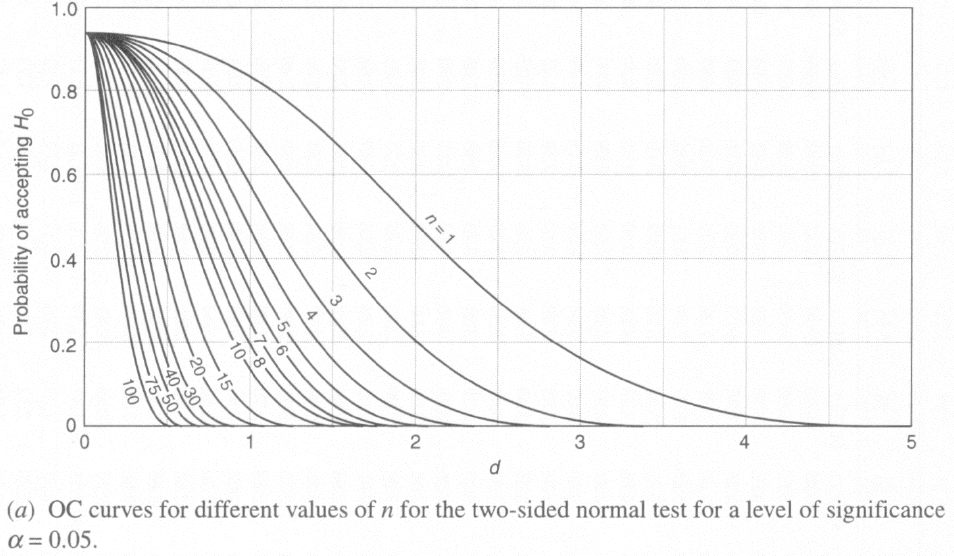
\includegraphics[width=\linewidth]{./images/rc5fig3.png}
\end{figure}

\end{frame}


\begin{frame}{Choosing the Sample Size}

\structb{More general case: OC curve.}
\begin{figure}[htbp]
	\centering
	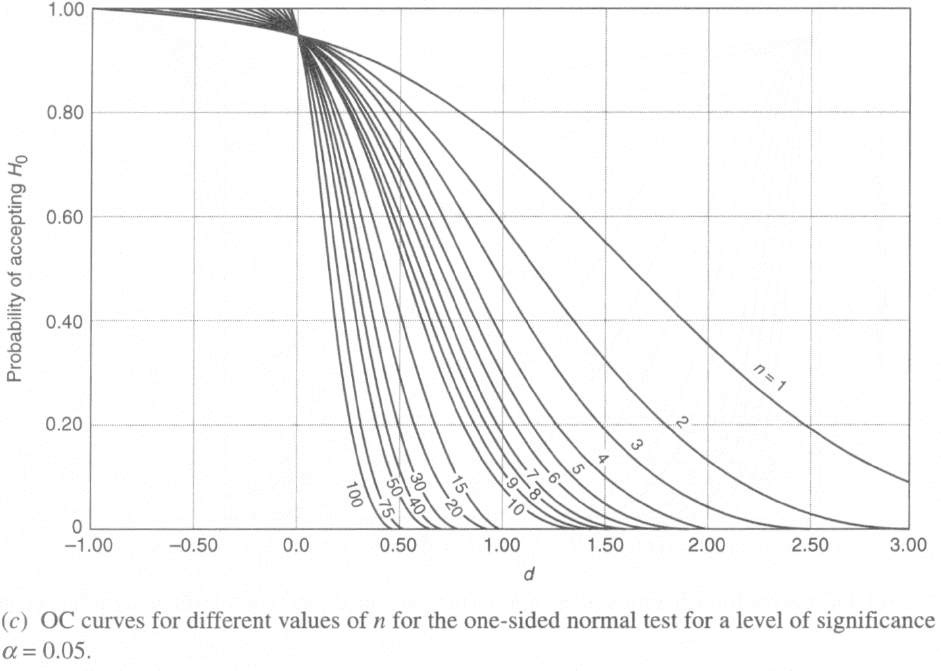
\includegraphics[width=\linewidth]{./images/rc5fig4.png}
\end{figure}

\end{frame}


\begin{frame}{Choosing the Critical Region}

\justifying
\structb{Determine the critical region using $\alpha$ and $n$.} The \highlightg{critical region} is chosen so that if $H_0$ is true, then the probability of test statistic's value falling into the critical region is no more than $\alpha$. \\
~\\
\structb{Critical region for mean.} Suppose the sample mean $\overline{X}$ follows a normal distribution with unknown mean $\mu$ and known variance $\sigma^2$, with $H_0: \mu = \mu_0$. Then the test statistic
\begin{align*}
Z = \frac{\overline{X} - \mu_0}{\sigma/\sqrt{n}} \sim \U{N}(0, 1),
\end{align*}
and thus the critical region is obtained from
\begin{align*}
\frac{|\overline{X} - \mu_0|}{\sigma/\sqrt{n}} > z_{\alpha/2}.
\end{align*}
We reject $H_0$ at significance level $\alpha$ and accept $H_1$ if $\overline{X}$ falls in this critical region.

\end{frame}

\begin{frame}{Neyman-Pearson Decision Theory}

\structb{Example.}

\end{frame}


\section{Test for Statistics}

\subsection{Tests for Mean, Median and Variance}

\subsection{Inferences on Proportions}


\subsection{Comparing Two Means and Two Variances}